\documentclass[conference]{IEEEtran}
\IEEEoverridecommandlockouts
% The preceding line is only needed to identify funding in the first footnote. If that is unneeded, please comment it out.
%Template version as of 6/27/2024

\usepackage{cite}
\usepackage{amsmath,amssymb,amsfonts}
\usepackage{algorithmic}
\usepackage{graphicx}
\usepackage{textcomp}
\usepackage{xcolor}
\def\BibTeX{{\rm B\kern-.05em{\sc i\kern-.025em b}\kern-.08em
    T\kern-.1667em\lower.7ex\hbox{E}\kern-.125emX}}
\begin{document}

\title{Chessy3D: A study of 3D Chessboard Detection and Pose Estimation\\
}

\author{\IEEEauthorblockN{Luca Villani}
\IEEEauthorblockA{
\textit{matr. 200412}\\
\textit{University of Modena and Reggio Emilia}\\
269419@studenti.unimore.it}
\and
\IEEEauthorblockN{Alessandro Mezzogori}
\IEEEauthorblockA{\textit{matr. } \\
\textit{University of Modena and Reggio Emilia}\\
271617@studenti.unimore.it}
\and
\IEEEauthorblockN{Davide Della Casa Venturelli}
\IEEEauthorblockA{\textit{matr. } \\
\textit{University of Modena and Reggio Emilia}\\
xxxxx@studenti.unimore.it}
}

\maketitle

\begin{abstract}
In this paper, we present a novel framework for chessboard corners detection
 and chess-pieces object detection. 
Our approach tackles the significant challenges posed by the variability
 of the photos taken of the chessboard and sizes, color and differences of the chess pieces.
We propose a new method for chessboard keypoint detection that utilizes a combination of
 deep learning and geometric constraints to accurately identify the keypoints on the chessboard
 and the squares within it.
This method is robust to variations in lighting, angle, and chessboard designs,
making it suitable for real-world applications.
Additionally, we developed a chess-piece object detection model that can accurately detect and classify chess pieces in various conditions.
Our study delves into the intricacies of chessboard detection, addressing the challenges of different chessboard designs and piece variations.
The proposed approach using YOLOv8 for chess-piece detection
 demonstrates superior performance in terms of accuracy and robustness compared to existing methods.
We used two datasets for training and testing our models: ChessRed2K and another small dataset found on Roboflow.
After the object detection we will propose a FEN annotation method for converting the chessboard state into a
 FEN (Forsyth-Edwards Notation) string, which is a standard notation for describing the state of a chess game.
Additionally we show a method for retrieving similar images using one hot encoding
 and a similarity search algorithm.
\end{abstract}

\section{Introduction}
The detection and analysis of keypoints in images have
become crucial tasks in the field of computer vision, with
applications ranging from object recognition and tracking
to augmented reality and autonomous driving.

Identifying corners in images is a fundamental
problem in computer vision, with applications in
object recognition, image stitching, and 3D reconstruction.
Chessboard detection is a specific case of keypoint detection
that has gained significant attention due to its
importance in camera calibration, pose estimation, and
robotics. The chessboard pattern provides a regular and
structured grid that can be easily detected and used to
estimate the camera's intrinsic and extrinsic parameters.
In this paper, we present an approach for chessboard corners detection
and chess-pieces object detection using deep learning
and geometric constraints. Our method is designed to
handle the challenges posed by the variability of chessboard
photos, including different lighting conditions, angles,
and chessboard designs.

We have been through a series of steps to achieve our goal:
\begin{itemize}
    \item We started with the chessboard corners detection, using a combination of deep learning and geometric constraints to accurately identify the keypoints on the chessboard.
    \item We then moved on to chessboard squares detection, which involves detecting the individual squares on the chessboard.
    \item Next, we focused on chess-pieces object detection, using YOLOv8 to detect and classify chess pieces in various conditions.
    \item After that, we developed a FEN annotation method for converting the chessboard state into a FEN string.
    \item Finally, we implemented an image similarity search method using one hot encoding and a similarity search algorithm.
    \item We also conducted a series of experiments to evaluate the performance of our approach, comparing it with existing methods and demonstrating its effectiveness in real-world scenarios.
\end{itemize}

We used two datasets for training and testing our models: ChessRed2K and another small dataset found on Roboflow.
The rest of the paper is organized as follows: 
\begin{itemize}
    \item Section II discusses the related work in chessboard detection and keypoint detection.
    \item Section III describes the proposed approach for chessboard corners detection.
    \item Section IV presents the chessboard squares detection method.
    \item Section V details the chess-pieces object detection using YOLOv8.
    \item Section VI explains the FEN annotation method.
    \item Section VII discusses the image similarity search method.
\end{itemize}



\section{Chessboard Corners Detection} - Davide

\section{Chessboard Squares Detection} - Davide

\section{Chess-Pieces Object Detection} - Luca
\usepackage{graphicx}

We initially approached the problem of chess-pieces object detection using DETR (Detection Transformer), with a ResNet-50 backbone, used for object detection tasks.
The DETR model was pre-trained on the COCO dataset and fine-tuned on a custom dataset of 2000 chess images, which included various chess pieces in different lighting conditions,
 angles, and designs annotated in the COCO format with 12 classes representing the different chess pieces (e.g., white-pawn, white-knight, white-bishop, etc.).
However, we encountered several challenges with this method, particularly in terms of performance and accuracy.
Despite tuning and training the model for 100, 150 and 200 epoch, DETR consistently underperformed.
The DETR model struggled with the variability of chess pieces in different lighting conditions, angles, and designs, leading to suboptimal detection results.
We found out that the model was not able to converge properly, and the loss function did not decrease as expected during training.
This led us to explore alternative approaches for chess-piece object detection.

We then turned our attention to YOLOv8, a state-of-the-art object detection model that has shown promising results in various applications.
We trained YOLOv8 on the same custom dataset of 2000 chess images, which included various chess pieces in different lighting conditions, angles, and designs.
The training process was more successful with YOLOv8, as the model was able to converge properly and achieve a lower loss function.
The YOLOv8 model demonstrated superior performance in terms of accuracy and robustness compared to DETR.

The model was trained from a pre-trained checkpoint found online and fine-tuned on our custom dataset.[ref to github repo]
We conducted three training runs with different parameters like:
\begin{itemize}
    \item Data augmentations (mosaic augmentation)
    \item HSV shifts
    \item Horizontal and vertical flips
\end{itemize}
The training was performed using PyTorch 2.1 on an NVIDIA RTX 3090 GPU with 24GB of VRAM.

The three training runs were conducted with the two datasets in this order:
\begin{itemize}
    \item YOLOv8m run 1: A small dataset found on Roboflow, which contains 100 images of chess pieces in different lighting conditions and angles.
    \item YOLOv8m run 2: ChessRed2K dataset, which contains 2000 images of chess pieces in various conditions.
    \item YOLOv8m run 3: Starting from run 1 we used ChessRed2K dataset for finetuning the model.
\end{itemize}

The YOLOv8m model performed well, achieving a mean Average Precision (mAP) of
 approximately 0.87 at IoU threshold 0.5 and a
  mAP of approximately 0.77 at IoU thresholds from 0.5 to 0.95.

As we can see in the table below, the model achieved high precision
 and recall values across the three training runs,
indicating its effectiveness in detecting and classifying chess pieces.
All the runs showed converged approximately in 200 epochs.

\begin{table}[ht]
\centering
\caption{Key performance metrics for the three YOLOv8m training runs.}
\label{tab:YOLOv8-results}
\resizebox{\linewidth}{!}{%
\begin{tabular}{lccccl}
\toprule
\textbf{Run} & \textbf{Precision (B)} & \textbf{Recall (B)} & \textbf{mAP@0.5} & \textbf{mAP@0.5:0.95} \\
\midrule
YOLOv8m Run 1 & $\sim$0.88 & $\sim$0.93 & $\sim$0.87 & $\sim$0.75 \\
YOLOv8m Run 2 & $\sim$0.90 & $\sim$0.95 & $\sim$0.89 & $\sim$0.78 \\
YOLOv8m Run 3 & $\sim$0.87 & $\sim$0.91 & $\sim$0.85 & $\sim$0.72 \\
\bottomrule
\end{tabular}
}
\end{table}


In terms of loss behavior, we decided to use three different loss functions:
\begin{itemize}
    \item Classification Loss: it measures the accuracy of the model predictions in classfiying the class inside the bounding box.
    For this loss YOLOv8m uses a binary cross-entropy loss function.
    \item Box Loss: it measures the accuracy of the model in predicting bounding box positions and sizes. It's calculated with a combinantion of IoU (Interection over Union).
    \item Distribution Focal Loss: this loss function is an advanced feature of YOLOv8. It measures the accuracy of the model in identifying the presence of objects inside the image. It's used to handle better small objects.
\end{itemize}

\begin{table}[ht]
\centering
\caption{Final loss values for the three YOLOv8m runs. All values are approximate and taken at convergence (step $\sim$200).}
\label{tab:yolov8-loss}
\resizebox{\linewidth}{!}{%
\begin{tabular}{lccc}
\toprule
\textbf{Run} & \textbf{Classification Loss (cls\_loss)} & \textbf{Box Loss (box\_loss)} & \textbf{DFL Loss (dfl\_loss)} \\
\midrule
YOLOv8m Run 1 & $\sim$0.06 & $\sim$0.35 & $\sim$1.10 \\
YOLOv8m Run 2 & $\sim$0.05 & $\sim$0.32 & $\sim$1.05 \\
YOLOv8m Run 3 & $\sim$0.07 & $\sim$0.38 & $\sim$1.15 \\
\bottomrule
\end{tabular}
}
\end{table}

Compared to earlier training runs and attempts with DETR that showed high loss values and poor convergence, YOLOv8m performed significantly better in terms of loss values and detection robustness.
We decided to use the third run of YOLOv8m as our final model for chess-piece object detection, as it showed the best performance in terms of precision, recall, and mAP values.

\begin{figure}[ht]
\centering
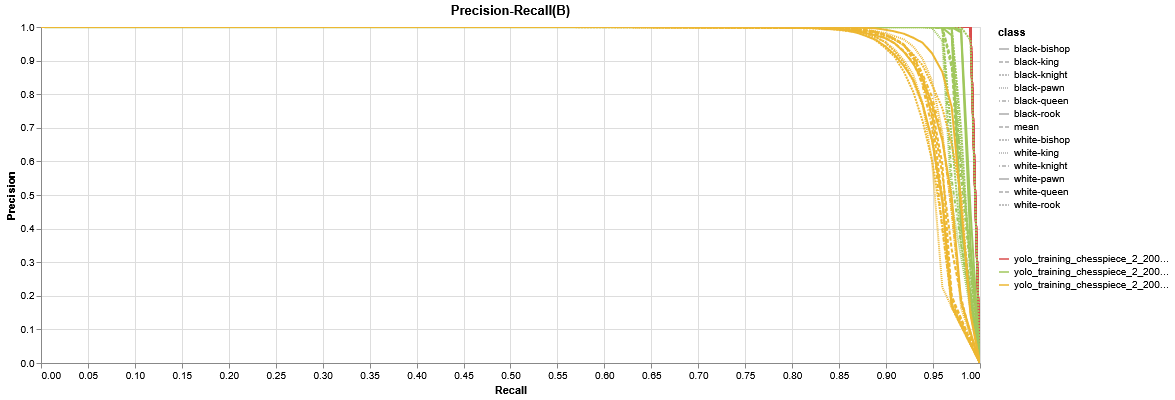
\includegraphics[width=\linewidth]{images/PR-runs-obj.png}
\caption{Precision-Recall curve for YOLOv8m. Yellow: Run 1, Green: Run 2, Red: Run 3. }
\label{fig:chess-detection}
\end{figure}


\section{FEN Annotation Method}  - Alle Luca
%% - common format used to share chess game state:
%% - Forsyth–Edwards Notation ( wiki definition )
%% - explanation

\subsection{What is FEN?} 
``FEN is the abbreviation of Forsyth-Edwards Notation, and it is the standard notation to describe positions of a chess game. Steven J. Edwards, a computer programmer, created this notation system based on another system designed by the journalist David Forsyth.`` 
\cite{chess:fen}
\newline
it allows easy storage and shareability of a position accounting for all the possible hidden states other than piece locations.

\subsection{Definition}
Composed by 6 ASCII strings separated by a space, each describes an aspect of the position.

\begin{itemize}
    \item {
        \textbf{Piece placement}: begins from the eigth rank and first file, describes the content of each square using lowercase letters for black, uppercase for white and numbers for empty squares.
        \begin{center}Initial position\end{center}
        \begin{center}
        \textit{rnbqkbnr/pppppppp/8/8/8/8/PPPPPPPP/RNBQKBNR}                    
        \end{center}
    }
    \item {
        \textbf{Active color}: who is going to move next, denoted by "w" or "b"
        \begin{center}
        \textit{rnbqkbnr/pppppppp/8/8/8/8/PPPPPPPP/RNBQKBNR w}                    
        \end{center}
    }
    \item {
        \textbf{Castling rights}: Uppercase letter comes first and indicates castleing right for white, followed by lowercased for black, "k" indicates king side is available, "q" means that a player may castle queenside
        \begin{center}
        \textit{rnbqkbnr/pppppppp/8/8/8/8/PPPPPPPP/RNBQKBNR w KQkq}                    
        \end{center}
    }
    \item {
        \textbf{Possible En Passant Targets}: if a pawn has moved two squares it is possible to capture en passant, if available the FEN adds the square behind the pawn in algebraic notation, else a "-"
        \begin{center}
        \textit{rnbqkbnr/pppppppp/8/8/8/8/PPPPPPPP/RNBQKBNR w KQkq -}                    
        \end{center}
    }
    \item {
        \textbf{Halfmove Clock}: Informs of how many moves both players have made since the last pawn advance or piece capture.
        \begin{center}
        \textit{rnbqkbnr/pppppppp/8/8/8/8/PPPPPPPP/RNBQKBNR w KQkq - 0}                    
        \end{center}
    }
    \item {
        \textbf{Fullmove Number}: Shows the number of completed turns in the game.
        \begin{center}
        \textit{rnbqkbnr/pppppppp/8/8/8/8/PPPPPPPP/RNBQKBNR w KQkq - 0 1}                    
        \end{center}
    }
\end{itemize}
The ease of understanding and simplicity of the format makes it trivial to implement a parser, 
thus allowing almost global use of the format across chess related software being the de factor standard to describe a chess position.




\section{Image Similarity Search} - Alle
%% - fen is not good for retrieval tasks ( variable ecc.. )
%% - approaches of other papers ( Inverted document index paper ) small mention
%% - general approach 
%%      - from position to embedding
%%      - embedding search
%% - naive approach chose
%% - possible other approaches ( if not long enough )

\subsection{Current state}
Although fen is a perfect medium for sharing, storing position and retrieving the exact match, 
due to its definition it makes comparison between similar but not equal positions using the format
difficult without parsing and loading both positions in memory, 
this becomes an hindrance especially when browsing chess databases to find games with similar position due to the computational cost of the operation.

The state of the art for storing and retrieving positions is varied based on the system that utilizes it.

SCID Shane's Chess Information Database one of the most famous tools used to find, navigate and study games, powerful but does not handle search by similarity.
Lichess, one of the main chess platforms, has a developed a highly efficient format \cite{retrieval:lichess:format} that allows search alike SCID.

This inability to allow search by similarity is mainly because of the hazy, subjective definition of similarity in games as it could be approached from different angles.
- Pure Positional similarity
- Threat similarity: attacking and defending pieces
- Structural similarity: in most games recurring piece structures are created

A novel approached is offered by Ganguly, Debasis and Leveling, Johannes and Jones, Gareth 
\cite{retrieval:soa:ids} that offers a novel approach by using information retrieval methods applied to a position.
in which they model a text representation of the position by utilizing positional information, square control, attacking and defending pieces.

In this project we utilized only positional information to build a pure piece positional index similarity.

\subsection{Project}
Goal: retrieving same or similar position to the given one

we opted for a pure positional information, Although using only the position of the pieces may return only apparently similar games with them being different because 
slight changes in position could lead to big difference in play, the approach is valid to explore the problem and given a sufficiently large database it will return 
games in which the position or a position less than two move difference.

by encoding the position in a naive binary embedding of 64 slot of length 12 where the first 6 bits represent the white pieces and the other 6 bits the black pieces, 

1..
2..
3..

%% image of a chess piece to an slice of embedding

we can build an exact one to one embedding of positional information of the reached position.

ALGORITMO
\dots
\dots

\subsection{Search}
The search and retrieval of the embeddings is efficiently done trough an hamming distance HNSW index, that enables 
ranking positions based on the number of flipped bits compared to the anchor embedding.
in a general we observed that for each 2 unit distances it corresponds to a different piece position, this could be intuitively understood 
by seeing it as toggling squares, a distance of 2 means a toggle off of one square 
%% show image %%
and a toggle on of another square.
pay attention that this intuition does not generalize in case of captures, castling, en passant... that involve more than one piece moves.

by following this approach we were able to construct a chess game database based on LumbrasGigabase \cite{retrieval:lumbrasgigabase} of 15 million games, 
and approximately 750 million chess positions but due to hardware memory and computation limitations we had to scale the indexing of the positions to allow only 5 million instances.

\subsection{Retrieval database construction}
the LumbrasGigabase offers games in PGN, portable game notation, that uses a combination of metadata, FEN notation and algebraic notation to describe 
respectively information about the game, like players, events and such, the starting position and following moves of a games.

%% example pgn format

by iterating over each game we extract and processed each position by creating and embedding and an hash to efficiently store the same position used in different games.
the hash used is a standard chess position hash called Zobrist hashing \cite{retrieval:zobristhash} that returns a 64bit unsigned integer value.


%% SOA METHODS https://arxiv.org/html/2310.04086v3 BIBTEX: https://arxiv.org/html/2310.04086v3/#bib.bibx15

\section{Conclusion} - Luca



\begin{thebibliography}{00}
\bibitem{b1} G. Eason, B. Noble, and I. N. Sneddon, ``On certain integrals of Lipschitz-Hankel type involving products of Bessel functions,'' Phil. Trans. Roy. Soc. London, vol. A247, pp. 529--551, April 1955.
\bibitem{b2} J. Clerk Maxwell, A Treatise on Electricity and Magnetism, 3rd ed., vol. 2. Oxford: Clarendon, 1892, pp.68--73.
\bibitem{b3} I. S. Jacobs and C. P. Bean, ``Fine particles, thin films and exchange anisotropy,'' in Magnetism, vol. III, G. T. Rado and H. Suhl, Eds. New York: Academic, 1963, pp. 271--350.
\bibitem{b4} K. Elissa, ``Title of paper if known,'' unpublished.
\bibitem{b5} R. Nicole, ``Title of paper with only first word capitalized,'' J. Name Stand. Abbrev., in press.
\bibitem{b6} Y. Yorozu, M. Hirano, K. Oka, and Y. Tagawa, ``Electron spectroscopy studies on magneto-optical media and plastic substrate interface,'' IEEE Transl. J. Magn. Japan, vol. 2, pp. 740--741, August 1987 [Digests 9th Annual Conf. Magnetics Japan, p. 301, 1982].
\bibitem{b7} M. Young, The Technical Writer's Handbook. Mill Valley, CA: University Science, 1989.
\bibitem{b8} D. P. Kingma and M. Welling, ``Auto-encoding variational Bayes,'' 2013, arXiv:1312.6114. [Online]. Available: https://arxiv.org/abs/1312.6114
\bibitem{b9} S. Liu, ``Wi-Fi Energy Detection Testbed (12MTC),'' 2023, gitHub repository. [Online]. Available: https://github.com/liustone99/Wi-Fi-Energy-Detection-Testbed-12MTC
\bibitem{b10} ``Treatment episode data set: discharges (TEDS-D): concatenated, 2006 to 2009.'' U.S. Department of Health and Human Services, Substance Abuse and Mental Health Services Administration, Office of Applied Studies, August, 2013, DOI:10.3886/ICPSR30122.v2
\bibitem{b11} K. Eves and J. Valasek, ``Adaptive control for singularly perturbed systems examples,'' Code Ocean, Aug. 2023. [Online]. Available: https://codeocean.com/capsule/4989235/tree
\end{thebibliography}

\vspace{12pt}
\end{document}








